\documentclass{beamer}
\usetheme{Median}
\title{IIR Filter IP}
\date{\today}
\author{Kevin Bloom}
\institute{Pennsylvania College of Technology}

%% \setbeamrecovered{invisible}
\setbeamercovered{%
  again covered={\opaqueness<1->{50}}}
\begin{document}

\maketitle

\section{Overview}
\begin{frame}{Overview}
  \begin{itemize}[<+>]
  \item System Design
  \item IIR IP
  \item Zynq Communication
  \item Example Outputs
  \end{itemize}
\end{frame}

\section{System Design}
\begin{frame}{System Design}
  Picture of the entire system, zoom in to see/explain things.
\end{frame}

\section{IIR IP}
\begin{frame}{IIR IP}
  This frame will contain a picture of the IP. Discuss the I/O pins.
\end{frame}
\begin{frame}{IIR IP --- Data Input Process }
  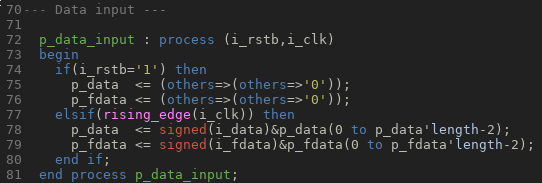
\includegraphics[height=3.5cm]
                  {data-input.png}
\end{frame}
\begin{frame}{IIR IP --- Arithmetic}
  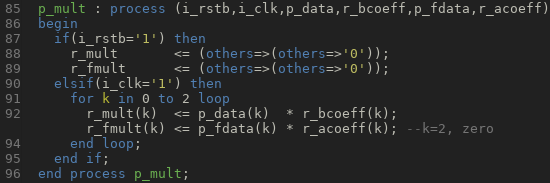
\includegraphics[height=3.5cm]
                  {mult.png}
\end{frame}
\begin{frame}{IIR IP --- Arithmetic}
  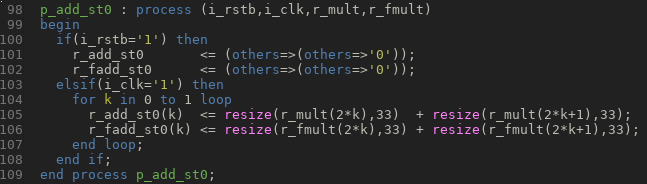
\includegraphics[height=3cm]
                  {add0.png}
\end{frame}
\begin{frame}{IIR IP --- Arithmetic}
  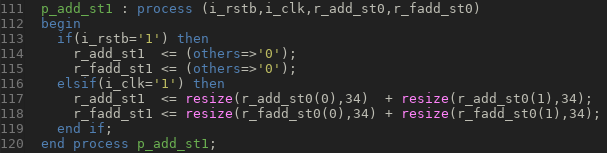
\includegraphics[height=2.5cm]
                  {add1.png}
\end{frame}
\begin{frame}{IIR IP --- Arithmetic}
  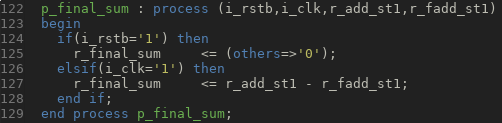
\includegraphics[height=2.5cm]
                  {final-add.png}
\end{frame}

\begin{frame}{IIR IP --- Data Output}
  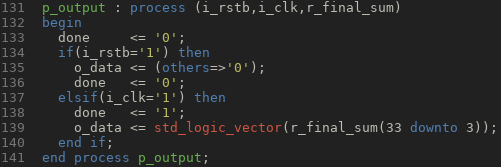
\includegraphics[height=3.5cm]
                  {output.png}
\end{frame}
\begin{frame}{IIR IP --- Elaborated Design }
  Big Picture, will need to zoom in.
\end{frame}
\begin{frame}{IIR IP --- IIR Troubles }
  \begin{itemize}[<+>]
  \item Single Stage vs BiQuad
  \item Floating Point to Fixed Point
  \item Gains and Scaling
  \end{itemize}
\end{frame}
\begin{frame}{IIR IP --- Single Stage Problems}
  \begin{columns}[T]
    \begin{column}[T]{5cm}
      \begin{itemize}[<+>]
      \item Number of coefficients increases dramatically
      \item Numerator coefficients approach zero
      \item Denominator coefficients approach infinity
      \end{itemize}
      \center{
        \visible<4->{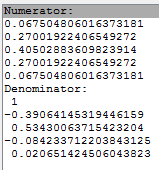
\includegraphics[height=2.5cm]
          {standard-coeffs-48kfs-10800fc.png}}}
    \end{column}
    \begin{column}[T]{5cm}
      \center{
        \visible<5->{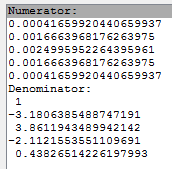
\includegraphics[height=2.5cm]
          {standard-coeffs-100kfs-5kfc.png}}
      \vspace{.08in}
      \visible<6->{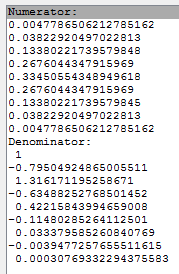
\includegraphics[height=4cm]
        {standard-coeffs-48kfs-10800fc-8order.png}}}
    \end{column}
  \end{columns}
\end{frame}
\begin{frame}{IIR IP --- BiQuad}
  \begin{columns}[T]
    \begin{column}[T]{5cm}
      \visible<1->{Pros}
      \begin{itemize}[<+>]
      \item Number of coefficients never change
      \item Small coefficient magnitudes
      \item Easy to make generic
      \end{itemize}
      \visible<4->{Cons}
      \begin{itemize}[<+>]
      \item Numerator coefficients need scaled
      \item Requires more hardware
      \end{itemize}
    \end{column}
    \begin{column}[T]{5cm}
      \visible<6->{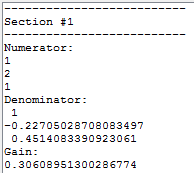
\includegraphics[height=3cm]
        {biquad-coeffs-section1-48kfs-10800fc.png}}
      \vfill
      \visible<6->{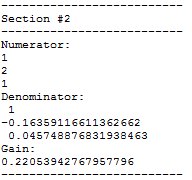
\includegraphics[height=3cm]
        {biquad-coeffs-section2-48kfs-10800fc.png}}
    \end{column}
  \end{columns}
\end{frame}
\begin{frame}{IIR IP --- Fixed Point}
  \center{
    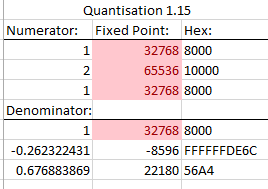
\includegraphics[height=5cm]
                  {overflow-coeffs.png}}
\end{frame}
\begin{frame}{IIR IP --- Scaling}
  \center{
    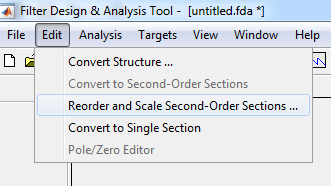
\includegraphics[height=5cm]
                    {scaling-location.png}
    }
\end{frame}
\begin{frame}{IIR IP --- Scaling}
  \center{
    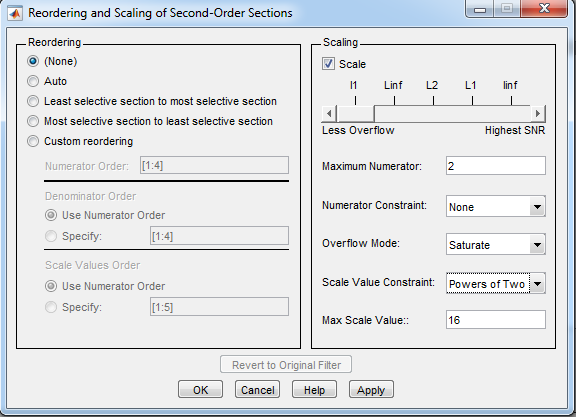
\includegraphics[height=7.5cm]
                    {scaled-window.png}
  }
\end{frame}
\begin{frame}{IIR IP --- Scaling}
  \begin{columns}[T]
    \begin{column}[T]{5cm}
      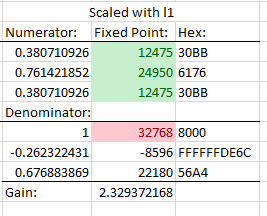
\includegraphics[height=4cm]
                      {scaled-with-l1.png}
    \end{column}
    \begin{column}[T]{5cm}
      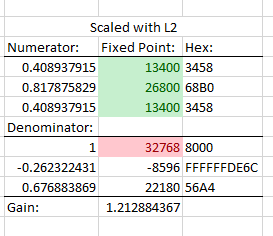
\includegraphics[height=4cm]
                      {scaled-with-L2.png}
    \end{column}
  \end{columns}
\end{frame}

\section{Zynq Communication}
\begin{frame}{Zynq Communication --- Outside the IP}
  Picture of the GPIOs that connect with the IPs, probably won't be using the
  mux/dmux design for this, so I'll be super basic. I might remove this entire
  section because it is so basic.
\end{frame}
\begin{frame}{Zynq Communication --- Inside the IP}
  Snippet of the coefficient input process
\end{frame}
\begin{frame}{Zynq Communication --- Inside the Zynq}
  Snippet of the coefficient input process
\end{frame}

\section{Example Outputs}
\begin{frame}{Example Outputs --- Lowpass}
  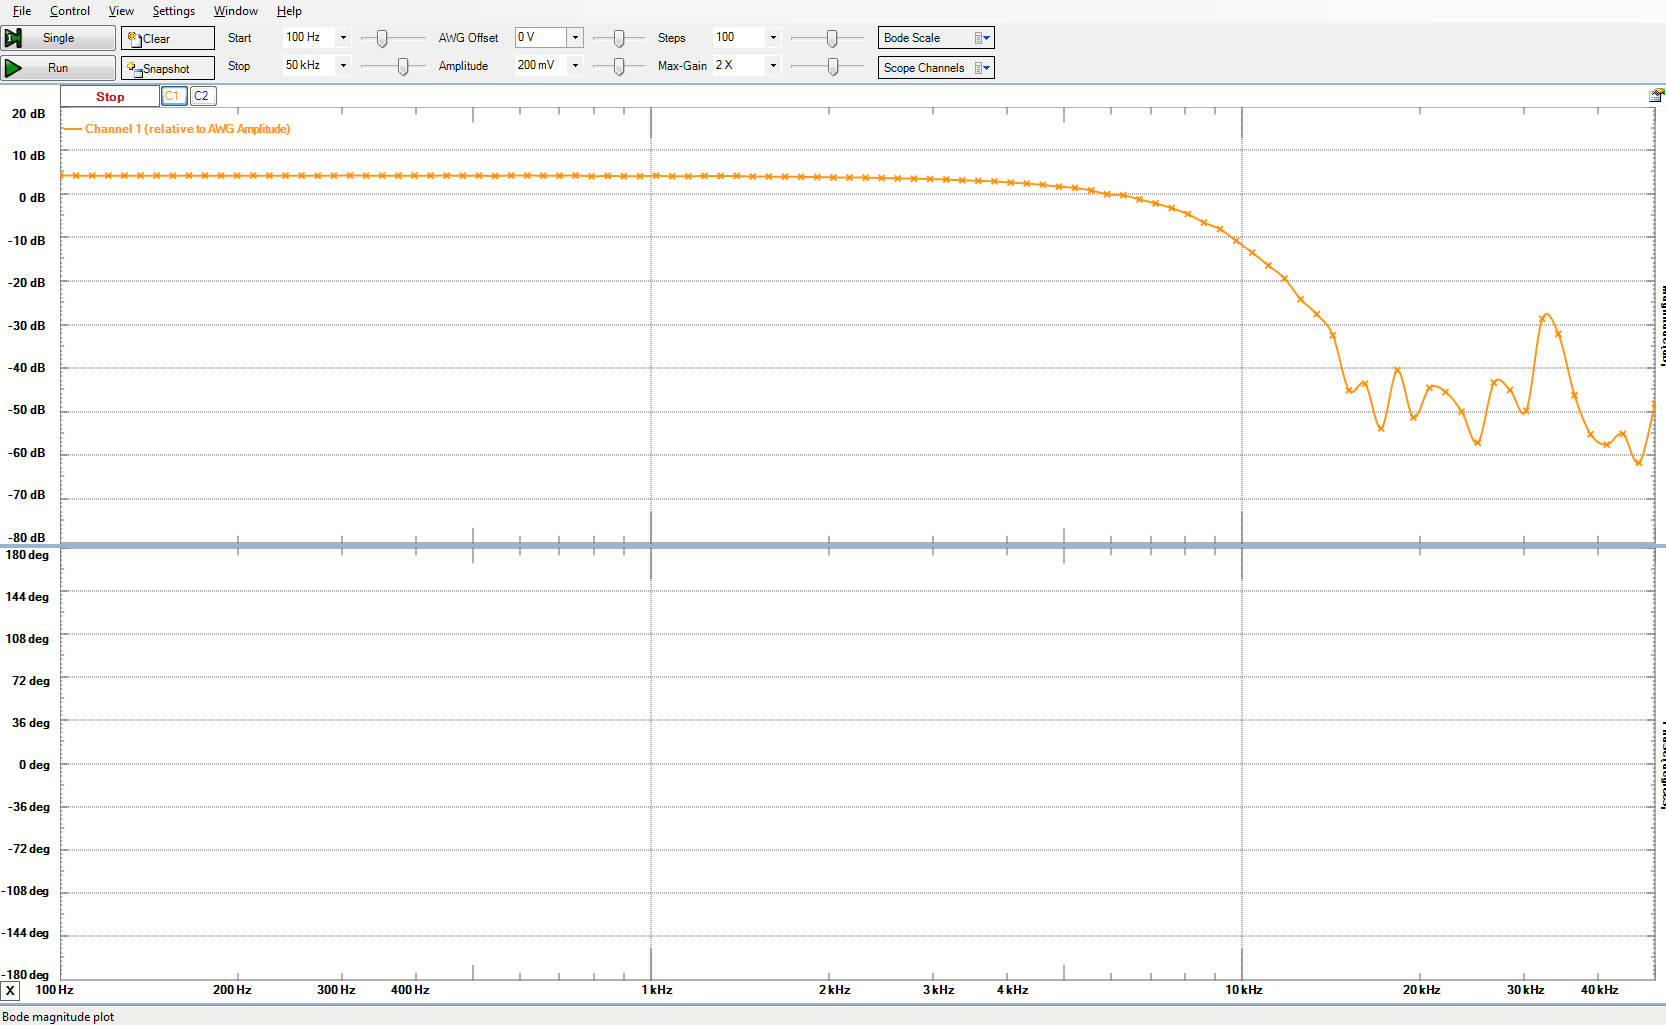
\includegraphics[height=6.5cm]
                  {very-nice-8th-order-lowpass.png}
\end{frame}
\begin{frame}{Example Outputs --- Highpass}
  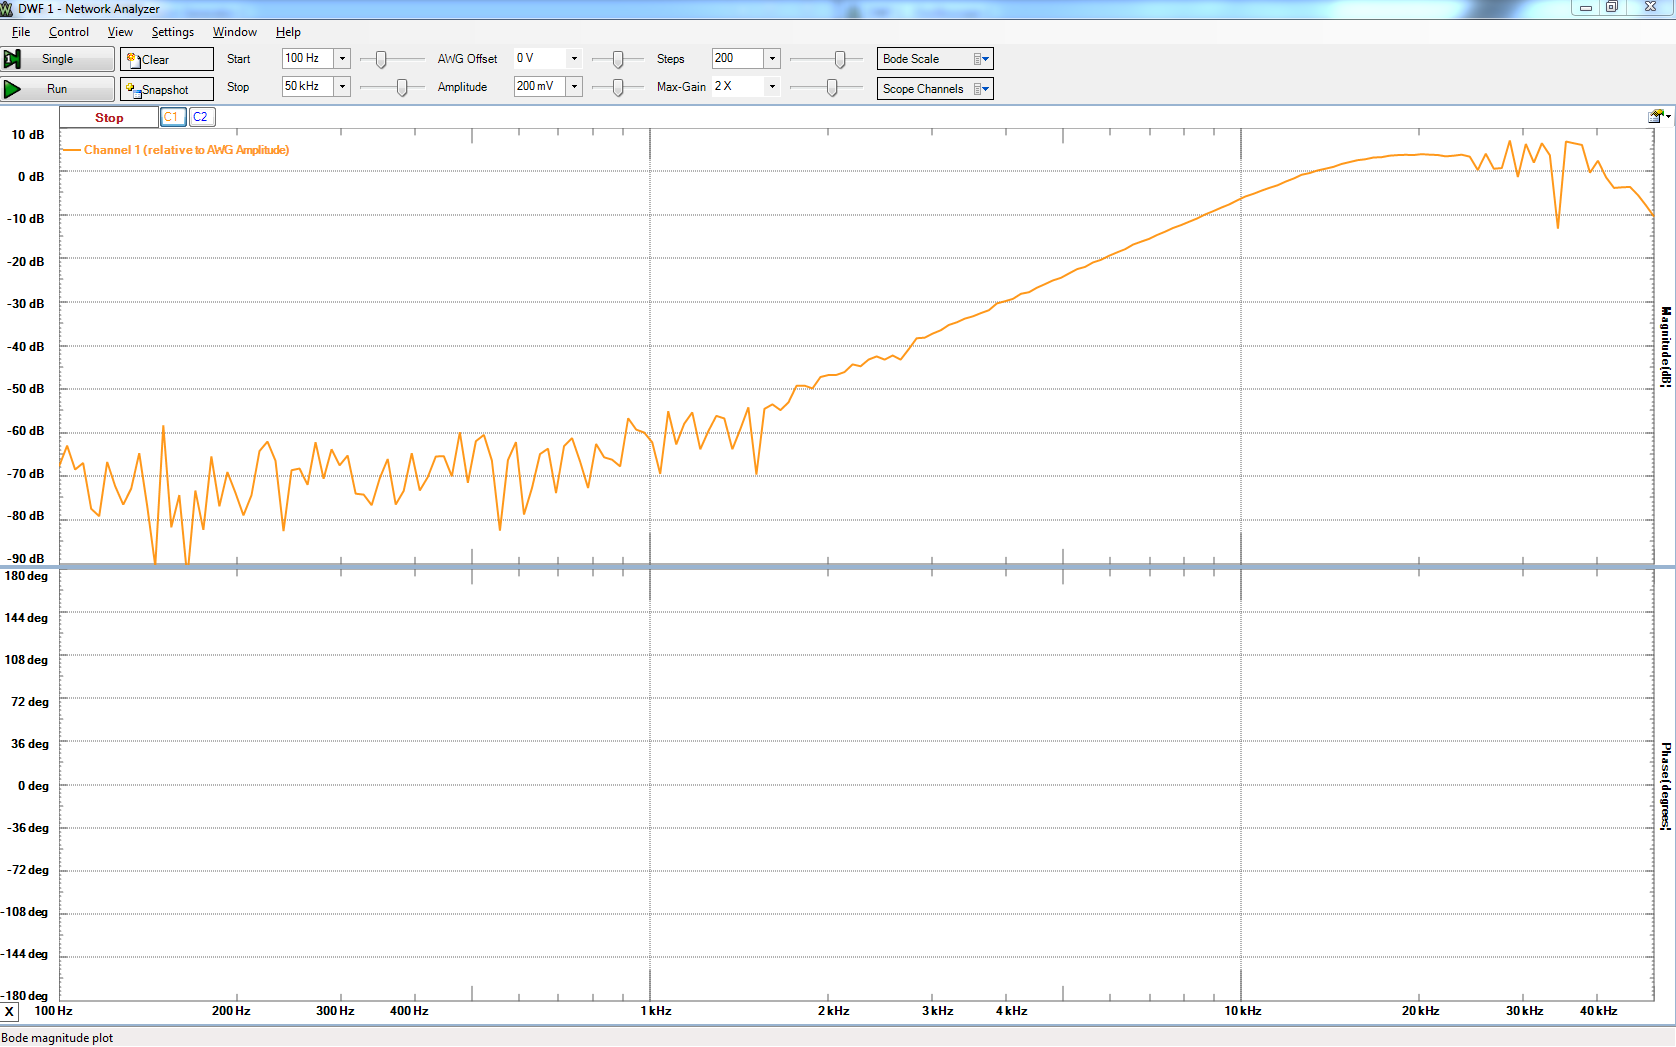
\includegraphics[height=6.5cm]
                  {iir-highpass-test2.png}
\end{frame}
\begin{frame}{Example Outputs --- Something Else}
  \includegraphics[height=6.5cm]
                  {iir-.png}
\end{frame}

\end{document}
